\documentclass[11pt]{article}
\usepackage{amsmath,textcomp,amssymb,geometry,graphicx,enumerate}
\usepackage{algorithm} % Boxes/formatting around algorithms
\usepackage[noend]{algpseudocode} % Algorithms
\usepackage{hyperref}
\hypersetup{
    colorlinks=true,
    linkcolor=blue,
    filecolor=magenta,      
    urlcolor=blue,
}

\def\Name{Matthew Wu}  % Your name
\def\SID{26604548}  % Your student ID number
%\def\Login{cs170-ajm} % Your login (your class account, cs170-xx)
\def\Homework{1} % Number of Homework
\def\Session{Spring 2017}

\title{CS 189 -- Spring 2017 --- Homework \Homework}
\author{\Name}%, SID \SID, \texttt{\Login}}
\markboth{CS 189--\Session\  Homework \Homework\ \Name}{CS 189--\Session\ Homework \Homework\ \Name}%, \texttt{\Login}}
\pagestyle{myheadings}
\date{}

\newenvironment{qparts}{\begin{enumerate}[{(}a{)}]}{\end{enumerate}}
\def\endproofmark{$\Box$}
\newenvironment{proof}{\par{\bf Proof}:}{\endproofmark\smallskip}

\textheight=9in
\textwidth=6.5in
\topmargin=-.75in
\oddsidemargin=0.25in
\evensidemargin=0.25in


\usepackage[utf8]{inputenc}

% Default fixed font does not support bold face
\DeclareFixedFont{\ttb}{T1}{txtt}{bx}{n}{8} % for bold
\DeclareFixedFont{\ttm}{T1}{txtt}{m}{n}{8}  % for normal

% Custom colors
\usepackage{color}
\definecolor{deepblue}{rgb}{0,0,0.5}
\definecolor{deepred}{rgb}{0.6,0,0}
\definecolor{deepgreen}{rgb}{0,0.5,0}

\usepackage{listings}

% Python style for highlighting
\newcommand\pythonstyle{\lstset{
language=Python,
basicstyle=\ttfamily\footnotesize,
otherkeywords={self},             % Add keywords here
keywordstyle=\ttb\color{deepblue},
emph={MyClass,__init__},          % Custom highlighting
emphstyle=\ttb\color{deepred},    % Custom highlighting style
stringstyle=\color{deepgreen},
frame=tb,                         % Any extra options here
showstringspaces=false           % 
}}


% Python environment
\lstnewenvironment{python}[1][]
{
\pythonstyle
\lstset{#1}
}
{}

% Python for external files
\newcommand\pythonexternal[2][]{{
\pythonstyle
\lstinputlisting[#1]{#2}}}

% Python for inline
\newcommand\pythoninline[1]{{\pythonstyle\lstinline!#1!}}


\begin{document}
\maketitle

\section*{1. Data Partitioning}
I select a random subset of data for a validation set by shuffling the data and then separating the first 10,000 rows of digits, the first 20\% rows of email feature vectors, and the first 5,000 rows of images from the rest. Before shuffling the email feature vectors, we combine the labels with the feature vectors without the labels.

\section*{2. Support Vector Machines}
First, I create a list of the number of training examples required. For each number $n$ of training examples, we take the first $n$ rows of the matrix with the training set, and train a linear classifier. The accuracy for each classifier is assessed by predicting the labels of the validation set, and calculating how close it is to the actual labels. The accuracy for each number of training points is kept in a list plotted in a graph. The generated plots are included below.\\

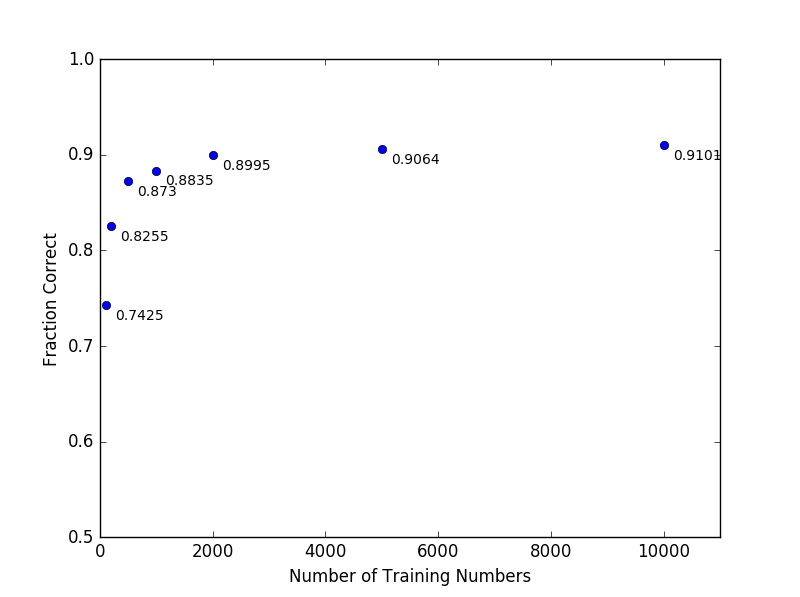
\includegraphics[scale=.7]{mnist_plot_2.png}\\

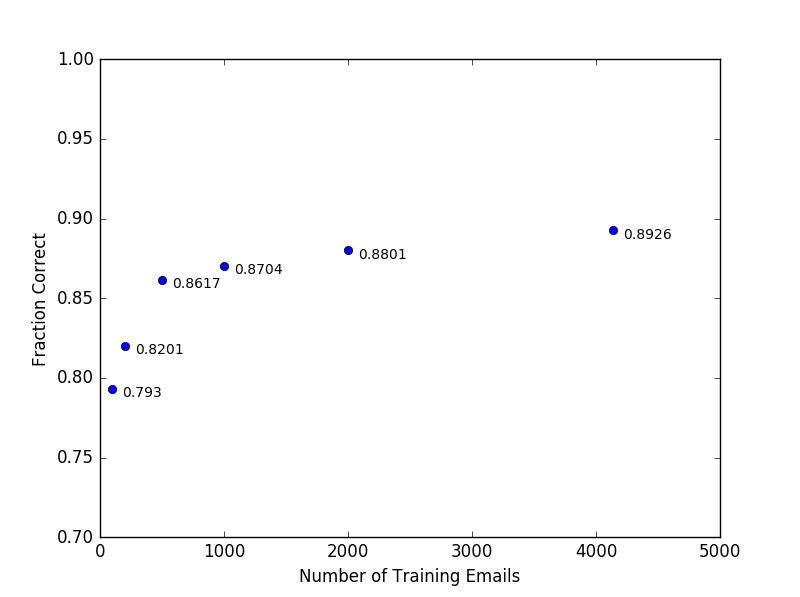
\includegraphics[scale=.7]{email_plot_2.png}\\

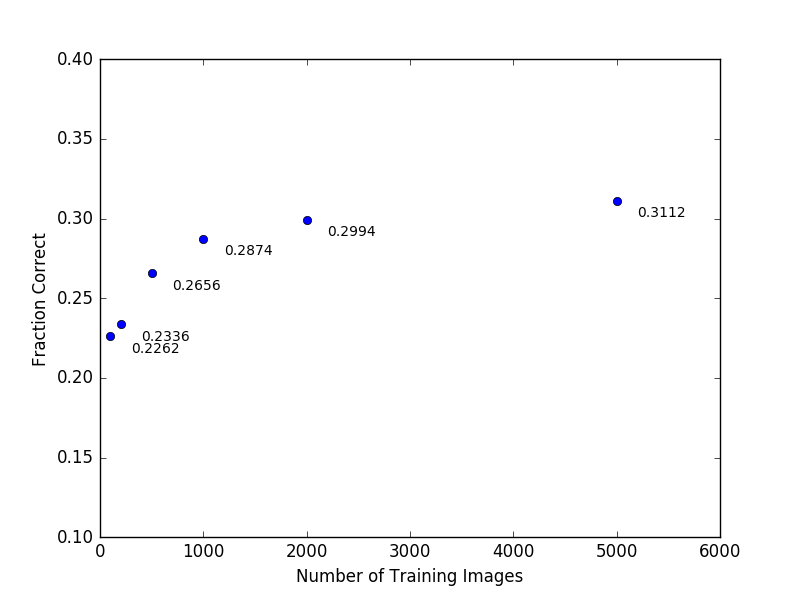
\includegraphics[scale=.7]{images_plot.png}

\newpage

\section*{3. Hyperparameter Tuning}
To quickly narrow down the optimal value for C to a narrower range, I initially only used 1000 training examples and powers of 10, specifically $10^x$ for integers $0 \leq x \leq 10$. From this preliminary test, it was easy to see that $10^0$ to around $10^{-5}$ made practically no difference, and everything below $10^{-7}$ was far worse than $C=1$. From this, I narrowed the optimal C value to be somewhere between $10^{-7}$ and $10^{-5}$. From there, I switched to using 10000 training examples, and I made a plot for the accuracy for several values of C. Depending on the validation set and training examples, different values of C performed better. I ended up making submissions with $10^{-7}*100^{x/10}$ for $x=\{3, 4, 5, 6\}$. The two graphs below illustrate the variation in performance the randomly selected sets can cause.

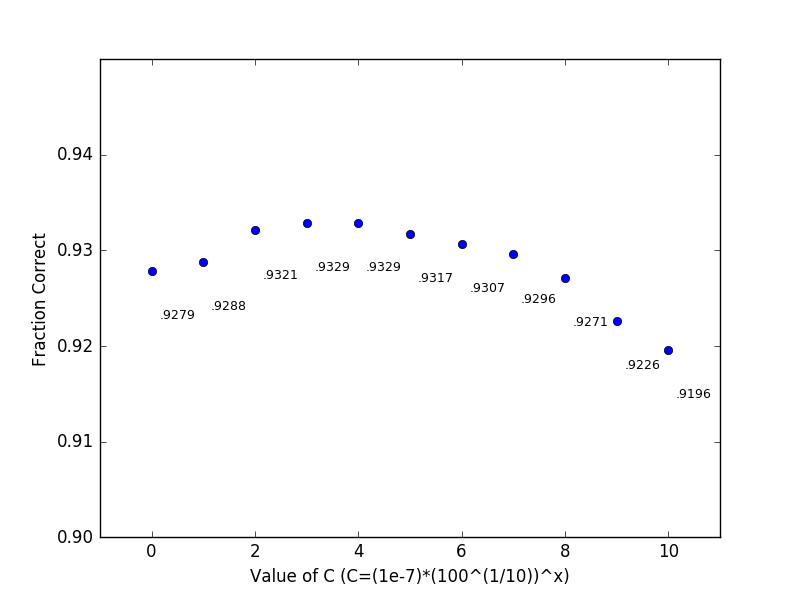
\includegraphics[scale=.55]{mnist_c_2.png}

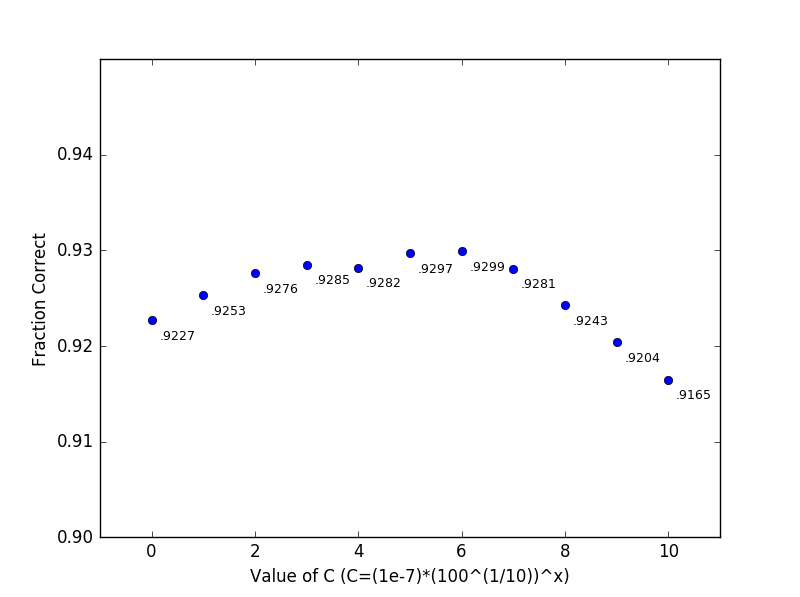
\includegraphics[scale=.55]{mnist_c_3.png}

\newpage

\section*{4. K-Fold Cross-Validation}
I used the built in KFold to perform k-fold cross validation for $C=\{.1, .3, 1, 3, 10\}$. Values of $C$ larger than 10 take too long to compute, and there were only minimal improvements for increasing $C$, so I settled on using $C=10$.

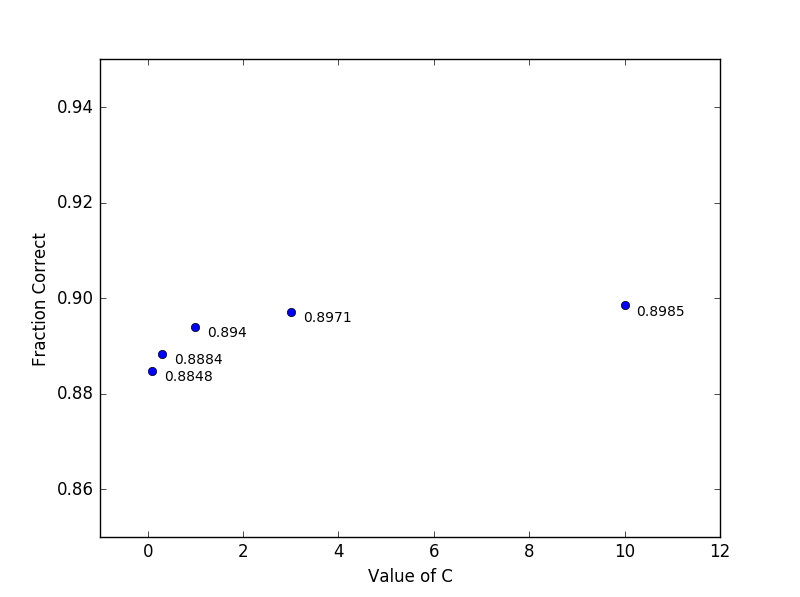
\includegraphics[scale=.7]{email_c_2.png}

\section*{5. Kaggle}
I used the optimal of $C$ computed from earlier and the entire training MNIST and email training sets to train the linear classifier.\\

My Kaggle score for MNIST was .94660.\\
My Kaggle score for spam was .88320.

\newpage
\section*{Appendix}
The following code was used to classify MNIST:
\begin{python}
import numpy as np
import scipy.io
import matplotlib.pyplot as plt
import csv

from sklearn.svm import SVC
from sklearn import metrics

traindatafilename = "hw01_data/mnist/train"
traindata = scipy.io.loadmat(traindatafilename)
traindata = traindata['trainX']

VAL_SIZE = 10000

np.random.shuffle(traindata)

validation = traindata[:VAL_SIZE]
training = traindata[VAL_SIZE:]

validation_data = validation[:,:-1]
temp = validation[:,784:]
validation_labels = temp.reshape(temp.shape[0])

def generate_plot():
    training_examples_list = [100, 200, 500, 1000, 2000, 5000, 10000]
    accuracy_list = []
    for num_training_examples in training_examples_list:
        training_set = training[:num_training_examples]
        x = training_set[:,:-1]
        y = training_set[:,784:]
        y = y.reshape(y.shape[0])
        classifier = SVC(kernel='linear')
        classifier.fit(x, y)
        guesses = classifier.predict(validation_data)
        score = metrics.accuracy_score(validation_labels, guesses)
        accuracy_list.append(score)

    plt.plot(training_examples_list, accuracy_list, 'bo')
    plt.axis([0, 11000, .5, 1])
    plt.ylabel("Fraction Correct")
    plt.xlabel("Number of Training Numbers")

    for i in range(7):
        text = str(accuracy_list[i])
        x = training_examples_list[i]
        y = accuracy_list[i]
        plt.annotate(text, xy = (x, y), xytext = (x + 160, y - .015), fontsize = 10)

    plt.show()

def find_c_value():
    #c_values = [10**-x for x in range(11)]
    #Everything from 10**0 to 10**-5 makes no difference
    #C=10**-6 is just barely better than C=1
    #C=10**-7 is just barely worse than C=1
    #C=10**-8 is significantly worse than C=1

    #The optimal value for C is likely between 10**-5 and 10**-7

    c_values = [(10**-7)*(100**(1/10))**x for x in range(11)]

    power_list = []
    accuracy_list = []

    for i in range(11):
        c = c_values[i]
        #num_training_examples = 1000
        num_training_examples = 10000
        training_set = training[:num_training_examples]
        x = training_set[:,:-1]
        y = training_set[:,784:]
        y = y.reshape(y.shape[0])
        classifier = SVC(kernel='linear', C = c)
        classifier.fit(x, y)
        guesses = classifier.predict(validation_data)
        score = metrics.accuracy_score(validation_labels, guesses)
        power_list.append(i)
        accuracy_list.append(score)
    plt.plot(power_list, accuracy_list, 'bo')
    plt.axis([-1, 11, .9, .95])
    plt.ylabel("Fraction Correct")
    plt.xlabel("Value of C (C=(1e-7)*(100^(1/10))^x)")

    for i in range(len(power_list)):
        text = str(accuracy_list[i])[1:]
        x = power_list[i]
        y = accuracy_list[i]
        plt.annotate(text, xy = (x, y), xytext = (x + .15, y - .002), fontsize = 9)

    plt.show()

def predict_test_set():
    c = 1e-7*(100**(1/10))**6
    x = traindata[:,:-1]
    y = traindata[:,784:]
    y = y.reshape(y.shape[0])
    classifier = SVC(kernel='linear', C = c)
    classifier.fit(x, y)
    testdatafilename = "hw01_data/mnist/test"
    testdata = scipy.io.loadmat(testdatafilename)
    testdata = testdata['testX']
    guesses = classifier.predict(testdata)
    with open('mnist_3.csv', 'w', newline='') as csvfile:
        writer = csv.writer(csvfile)
        writer.writerow(['Id', 'Category'])
        i = 0
        for g in guesses:
            writer.writerow([i, g])
            i += 1

generate_plot()
find_c_value()
predict_test_set()

\end{python}

\newpage
The following code was used to classify emails:
\begin{python}
import numpy as np
import scipy.io
import matplotlib.pyplot as plt
import csv

from sklearn.svm import SVC
from sklearn import metrics
from sklearn.cross_validation import KFold

traindatafilename = "hw01_data/spam/spam_data"
data = scipy.io.loadmat(traindatafilename)

traindata = data['training_data']
NUM_FEATURES = traindata.shape[1]
testdata = data['test_data']
labels = data['training_labels']
labels = labels.transpose()
traindata = np.append(traindata, labels, axis=1)
np.random.shuffle(traindata)

SIZE = traindata.shape[0]

def generate_plot():
    VAL_FRACTION = .2
    validation = traindata[:int(SIZE * VAL_FRACTION)]
    training = traindata[int(SIZE * VAL_FRACTION):]
    MAX_TRAIN_NUM = training.shape[0]
    validation_data = validation[:,:-1]
    temp = validation[:,NUM_FEATURES:]
    validation_labels = temp.reshape(temp.shape[0])
    training_examples_list = [100, 200, 500, 1000, 2000, MAX_TRAIN_NUM]
    accuracy_list = []
    for num_training_examples in training_examples_list:
        training_set = training[:num_training_examples]
        x = training_set[:,:-1]
        y = training_set[:,NUM_FEATURES:]
        y = y.reshape(y.shape[0])
        classifier = SVC(kernel='linear')
        classifier.fit(x, y)
        guesses = classifier.predict(validation_data)
        score = metrics.accuracy_score(validation_labels, guesses)
        accuracy_list.append(score)

    plt.plot(training_examples_list, accuracy_list, 'bo')
    plt.axis([0, 5000, .7, 1])
    plt.ylabel("Fraction Correct")
    plt.xlabel("Number of Training Emails")

    for i in range(6):
        text = str(round(accuracy_list[i], 4))
        x = training_examples_list[i]
        y = accuracy_list[i]
        plt.annotate(text, xy = (x, y), xytext = (x + 80, y - .005), fontsize = 10)

    plt.show()

def find_c_value():
    c_values = [.1, .3, 1, 3, 10]

    power_list = []
    accuracy_list = []

    kf = KFold(SIZE, n_folds=5)

    for c in c_values:
        total_score = 0
        for train_index, test_index in kf:
            training_set, validation_set = traindata[train_index], traindata[test_index]

            x = training_set[:,:-1]
            y = training_set[:,NUM_FEATURES:]
            y = y.reshape(y.shape[0])
            classifier = SVC(kernel='linear', C = c)
            classifier.fit(x, y)

            validation_data = validation_set[:,:-1]
            validation_labels = validation_set[:,NUM_FEATURES:]
            guesses = classifier.predict(validation_data)
            total_score += metrics.accuracy_score(validation_labels, guesses)

        score = total_score / 5
        power_list.append(c)
        accuracy_list.append(score)
    plt.plot(power_list, accuracy_list, 'bo')
    plt.axis([-1, 12, .85, .95])
    plt.ylabel("Fraction Correct")
    plt.xlabel("Value of C")

    for i in range(len(power_list)):
        text = str(round(accuracy_list[i], 4))
        x = power_list[i]
        y = accuracy_list[i]
        plt.annotate(text, xy = (x, y), xytext = (x + .25, y - .002), fontsize = 10)

    plt.show()

def predict_test_set():
    c = 10
    x = traindata[:,:-1]
    y = traindata[:,NUM_FEATURES:]
    y = y.reshape(y.shape[0])
    classifier = SVC(kernel='linear', C = c)
    classifier.fit(x, y)
    guesses = classifier.predict(testdata)
    with open('email.csv', 'w', newline='') as csvfile:
        writer = csv.writer(csvfile)
        writer.writerow(['Id', 'Category'])
        i = 0
        for g in guesses:
            writer.writerow([i, int(g)])
            i += 1

generate_plot()
find_c_value()
predict_test_set()
\end{python}
\newpage
The following code was used to add features to emails:
\begin{python}
'''
**************** PLEASE READ ***************

Script that reads in spam and ham messages and converts each training example
into a feature vector

Code intended for UC Berkeley course CS 189/289A: Machine Learning

Requirements:
-scipy ('pip install scipy')

To add your own features, create a function that takes in the raw text and
word frequency dictionary and outputs a int or float. Then add your feature
in the function 'def generate_feature_vector'

The output of your file will be a .mat file. The data will be accessible using
the following keys:
    -'training_data'
    -'training_labels'
    -'test_data'

Please direct any bugs to kevintee@berkeley.edu
'''

from collections import defaultdict
import glob
import re
import scipy.io

NUM_TRAINING_EXAMPLES = 5172
NUM_TEST_EXAMPLES = 5857

BASE_DIR = './'
SPAM_DIR = 'spam/'
HAM_DIR = 'ham/'
TEST_DIR = 'test/'

# ************* Features *************

# Features that look for certain words
def freq_pain_feature(text, freq):
    return float(freq['pain'])

def freq_private_feature(text, freq):
    return float(freq['private'])

def freq_bank_feature(text, freq):
    return float(freq['bank'])

def freq_money_feature(text, freq):
    return float(freq['money'])

def freq_drug_feature(text, freq):
    return float(freq['drug'] + freq['drugs'])

def freq_spam_feature(text, freq):
    return float(freq['spam'])

def freq_prescription_feature(text, freq):
    return float(freq['prescription'] + freq['prescript'])

def freq_creative_feature(text, freq):
    return float(freq['creative'])

def freq_height_feature(text, freq):
    return float(freq['height'])

def freq_featured_feature(text, freq):
    return float(freq['featured'])

def freq_differ_feature(text, freq):
    return float(freq['differ'])

def freq_width_feature(text, freq):
    return float(freq['width'])

def freq_other_feature(text, freq):
    return float(freq['other'])

def freq_energy_feature(text, freq):
    return float(freq['energy'])

def freq_business_feature(text, freq):
    return float(freq['business'])

def freq_message_feature(text, freq):
    return float(freq['message'])

def freq_volumes_feature(text, freq):
    return float(freq['volumes'])

def freq_revision_feature(text, freq):
    return float(freq['revision'])

def freq_path_feature(text, freq):
    return float(freq['path'])

def freq_meter_feature(text, freq):
    return float(freq['meter'])

def freq_memo_feature(text, freq):
    return float(freq['memo'])

def freq_planning_feature(text, freq):
    return float(freq['planning'])

def freq_pleased_feature(text, freq):
    return float(freq['pleased'])

def freq_record_feature(text, freq):
    return float(freq['record'])

def freq_out_feature(text, freq):
    return float(freq['out'])

# Features that look for certain characters
def freq_semicolon_feature(text, freq):
    return text.count(';')

def freq_dollar_feature(text, freq):
    return text.count('$')

def freq_sharp_feature(text, freq):
    return text.count('#')

def freq_exclamation_feature(text, freq):
    return text.count('!')

def freq_para_feature(text, freq):
    return text.count('(')

def freq_bracket_feature(text, freq):
    return text.count('[')

def freq_and_feature(text, freq):
    return text.count('&')

# --------- Add your own feature methods ----------
def empty_message(text, freq):
    if text == "Subject:":
        return 1
    return 0

def word_variance(text, freq):
    squared_total = 0
    total = 0
    for key, value in freq.items():
        squared_total += value**2
        total += value
    return squared_total / total

def long_words_at_end(text, freq):
    words = re.findall(r'[a-z]+', text)
    if len(words) <= 20:
        return 0
    total = 0
    for word in words[:20]:
        total += len(word)
    return total / 20

def freq_questions(text, freq):
    return float(freq['question'] + freq['questions'])

def freq_contact(text, freq):
    return float(freq['contact'] + freq['contacts'])

def freq_respond(text, freq):
    return float(freq['respond'])

def freq_picture(text, freq):
    return float(freq['picture'] + freq['pictures'])

def freq_attach(text, freq):
    return float(freq['attach'] + freq['attached'] + freq['attachment'])

def freq_one_letter_words(text, freq):
    num = 0
    for letter in 'bcdfghjklmnopqrstuvwxyz':
        num += freq[letter]
    return float(num)

def freq_html(text, freq):
    return float(freq['hmtl'])

def freq_com(text, freq):
    return float(freq['com'])

def freq_www(text, freq):
    return float(freq['www'])

def freq_net(text, freq):
    return float(freq['net'])

def freq_font(text, freq):
    return float(freq['font'])

def freq_bad_html(text, freq):
    return float(freq['bgcolor'] + freq['ffffff'] + freq['charset'] + freq['br'])

def freq_download(text, freq):
    return float(freq['download'] + freq['downloads'])

def freq_internet(text, freq):
    return float(freq['internet'])

def obviously_a_nigerian_prince(text, freq):
    num = freq['usd']
    num += freq['assist']
    num += freq['foreigner']
    num += freq['risk']
    num += freq['bank'] + freq['banking'] + freq['banks']
    num += freq['money']
    num += freq['00']
    num += freq['000']
    num += freq['transfer']
    num += freq['account'] + freq['accounts']
    num += freq['urgent'] + freq['urgently']
    num += freq['manager'] + freq['lawyer']
    num += freq['$']
    num += freq['offshore'] + freq['overseas'] + freq['oil']
    num += freq['invest'] + freq['investment'] + freq['investments']
    num += freq['million']
    return float(num)

def freq_credit(text, freq):
    return float(freq['credit'])

def freq_biz(text, freq):
    return float(freq['biz'])

def freq_gold(text, freq):
    return float(freq['gold'])

def freq_otp(text, freq):
    return float(freq['ship'] + freq['shipping'] + freq['ships'])

def freq_casino(text, freq):
    return float(freq['casino'])

def freq_hi_billy_mays_here(text, freq):
    return float(freq['guarantee'] + freq['guarantees'] + freq['guaranteed'])

def freq_advertise(text, freq):
    return float(freq['advertisement'] + freq['advertise'] + freq['ads'] + freq['ad'])

def freq_usd(text, freq):
    return float(freq['usd'] + freq['dollar'] + freq['dollars'])

def freq_cash(text, freq):
    return float(freq['cash'])

def freq_assist(text, freq):
    return float(freq['assist'])

def freq_risk(text, freq):
    return float(freq['risk'] + freq['risks'])

def freq_mortgage(text, freq):
    return float(freq['mortgage'] + freq['mortgages'])

def freq_interest_rate(text, freq):
    return float(min(freq['interest'], freq['rate'] + freq['rates']))

def freq_stock(text, freq):
    return float(freq['stock'] + freq['stocks'])

def freq_viagra(text, freq):
    return float(freq['viagra'] + freq['cialis'])

def freq_ummm(text, freq):
    num = 2 * min(freq['enlarge'] + freq['enlargement'], freq['pill'] + freq['pills'])
    num += freq['penis'] + freq['penises']
    num += freq['dick'] + freq['dicks']
    num += freq['cock'] + freq['cocks']
    num += freq['lubricant'] + freq['lube']
    num += freq['erect'] + freq['erection'] + freq['erections']
    num += freq['hardness']
    num += freq['arouse'] + freq['aroused'] + freq['arousal']
    num += freq['growth']
    return float(num)

def freq_pill(text, freq):
    return float(freq['pill'] + freq['pills'])

def freq_body_build(text, freq):
    num = freq['hormone']
    num += freq['hgh']
    num += freq['muscle']
    num += freq['mass']
    num += freq['fat']
    num += freq['body']
    return float(num)

def freq_dose(text, freq):
    return float(freq['dose'] + freq['mg'])

def freq_meet(text, freq):
    return float(freq['meet'] + freq['meeting'] + freq['meetings'])

def freq_medication(text, freq):
    return float(freq['medication'] + freq['medications'] + freq['meds'] + freq['rx'])

def freq_side_effect(text, freq):
    return float(min(freq['side'], freq['effect'] + freq['effects']) + 
        freq['sideeffects'] + freq['sideeffect'])

def freq_porn(text, freq):
    return text.count('porn')

def freq_sex(text, freq):
    return float(freq['sex'] + freq['sexy'] + freq['sexual'] +
        freq['orgy'] + freq['orgies'] +
        freq['fuck'] + freq['fucks'] + freq['fucker'])

def freq_dating(text, freq):
    num = freq['single'] + freq['singles']
    num += freq['flirt']
    num += freq['dating']
    return float(num)

def freq_orgasm(text, freq):
    return float(freq['orgasm'] + freq['orgasms'] + freq['intimate'] + freq['intimacy'])

def freq_buy(text, freq):
    return float(freq['buy'] + freq['buys'] + freq['order'] + freq['orders'])

def freq_deal(text, freq):
    return float(freq['deal'] + freq['deals'])

def freq_sale(text, freq):
    return float(freq['sale'] + freq['sales'])

def freq_offer(text, freq):
    return float(freq['offer'] + freq['offers'])

def freq_discount(text, freq):
    return float(freq['discount'] + freq['discounts'])

def freq_cheap(text, freq):
    return float(freq['cheap'])

def freq_low_prices(text, freq):
    return float(min(freq['low'] + freq['lowest'], freq['price'] + freq['prices']))

def freq_bonus(text, freq):
    return float(freq['bonus'] + freq['bonuses'])

def freq_mailing_list(text, freq):
    return float(freq['remove'] + freq['removed'] + freq['removal'] +
        freq['list'] + freq['unsubscribe'] + freq['unsubscription'] + freq['stop'] +
        freq['discontinue'] + 2 * min(freq['click'], freq['link'] + freq['here']))

def freq_discontinue(text, freq):
    return float(freq['discontinue'])

def freq_computron(text, freq):
    return float(freq['computron'])

def freq_weight(text, freq):
    num = freq['weight'] + freq['weigh'] + freq['loss'] + freq['lose']
    num += freq['fat'] + freq['burn'] + freq['burns']
    num += freq['calorized'] + freq['calories']
    return float(num)

def freq_weight_loss(text, freq):
    return float(min(freq['weight'] + freq['weigh'], freq['loss'] + freq['lose']))

def freq_wrinkle(text, freq):
    return float(freq['wrinkle'] + freq['wrinkles'])

def freq_diet(text, freq):
    return float(freq['diet'] + freq['diets'] + freq['dieting'])

def freq_trial(text, freq):
    return float(freq['trial'])

def freq_violence(text, freq):
    num = freq['explosion'] + freq['explosions'] + freq['explosives'] + freq['explosive']
    num += freq['detonate'] + freq['detonated']
    num += freq['troops'] + freq['troop'] + freq['soldier'] + freq['soldiers']
    num += freq['weapon'] + freq['weapons'] + freq['gun'] + freq['guns']
    num += freq['mortar'] + freq['shell'] + freq['shells'] + freq['bomb'] + freq['bombs']
    num += freq['military'] + freq['tank'] + freq['forces']
    return float(num)

def freq_question(text, freq):
    return text.count('?')

def freq_dash(text, freq):
    return text.count('-')

def freq_percent(text, freq):
    return text.count('%')

def freq_brace(text, freq):
    return text.count('{')

def duplicate_letters(text, freq):
    num = 0
    for i in range(1, len(text)):
        if text[i] == text[i-1]:
            num += 1
    return num / len(text)

# Generates a feature vector
def generate_feature_vector(text, freq):
    feature = []
    feature.append(freq_pain_feature(text, freq))
    feature.append(freq_private_feature(text, freq))
    feature.append(freq_bank_feature(text, freq))
    feature.append(freq_money_feature(text, freq))
    feature.append(freq_drug_feature(text, freq))
    feature.append(freq_spam_feature(text, freq))
    feature.append(freq_prescription_feature(text, freq))
    feature.append(freq_creative_feature(text, freq))
    feature.append(freq_height_feature(text, freq))
    feature.append(freq_featured_feature(text, freq))
    feature.append(freq_differ_feature(text, freq))
    feature.append(freq_width_feature(text, freq))
    feature.append(freq_other_feature(text, freq))
    feature.append(freq_energy_feature(text, freq))
    feature.append(freq_business_feature(text, freq))
    feature.append(freq_message_feature(text, freq))
    feature.append(freq_volumes_feature(text, freq))
    feature.append(freq_revision_feature(text, freq))
    feature.append(freq_path_feature(text, freq))
    feature.append(freq_meter_feature(text, freq))
    feature.append(freq_memo_feature(text, freq))
    feature.append(freq_planning_feature(text, freq))
    feature.append(freq_pleased_feature(text, freq))
    feature.append(freq_record_feature(text, freq))
    feature.append(freq_out_feature(text, freq))
    feature.append(freq_semicolon_feature(text, freq))
    feature.append(freq_dollar_feature(text, freq))
    feature.append(freq_sharp_feature(text, freq))
    feature.append(freq_exclamation_feature(text, freq))
    feature.append(freq_para_feature(text, freq))
    feature.append(freq_bracket_feature(text, freq))
    feature.append(freq_and_feature(text, freq))

    # --------- Add your own features here ---------
    # Make sure type is int or float

    feature.append(empty_message(text, freq))
    feature.append(word_variance(text, freq))
    feature.append(long_words_at_end(text, freq))
    feature.append(freq_questions(text, freq))
    feature.append(freq_contact(text, freq))
    feature.append(freq_respond(text, freq))
    feature.append(freq_picture(text, freq))
    feature.append(freq_attach(text, freq))
    feature.append(freq_one_letter_words(text, freq))
    feature.append(freq_html(text, freq))
    feature.append(freq_com(text, freq))
    feature.append(freq_www(text, freq))
    feature.append(freq_net(text, freq))
    feature.append(freq_font(text, freq))
    feature.append(freq_bad_html(text, freq))
    feature.append(freq_download(text, freq))
    feature.append(freq_internet(text, freq))
    feature.append(obviously_a_nigerian_prince(text, freq))
    feature.append(freq_credit(text, freq))
    feature.append(freq_biz(text, freq))
    feature.append(freq_gold(text, freq))
    feature.append(freq_otp(text, freq))
    feature.append(freq_casino(text, freq))
    feature.append(freq_hi_billy_mays_here(text, freq))
    feature.append(freq_advertise(text, freq))
    feature.append(freq_usd(text, freq))
    feature.append(freq_cash(text, freq))
    feature.append(freq_assist(text, freq))
    feature.append(freq_risk(text, freq))
    feature.append(freq_mortgage(text, freq))
    feature.append(freq_interest_rate(text, freq))
    feature.append(freq_stock(text, freq))
    feature.append(freq_viagra(text, freq))
    feature.append(freq_ummm(text, freq))
    feature.append(freq_pill(text, freq))
    feature.append(freq_body_build(text, freq))
    feature.append(freq_dose(text, freq))
    feature.append(freq_meet(text, freq))
    feature.append(freq_medication(text, freq))
    feature.append(freq_side_effect(text, freq))
    feature.append(freq_porn(text, freq))
    feature.append(freq_sex(text, freq))
    feature.append(freq_dating(text, freq))
    feature.append(freq_orgasm(text, freq))
    feature.append(freq_buy(text, freq))
    feature.append(freq_deal(text, freq))
    feature.append(freq_sale(text, freq))
    feature.append(freq_offer(text, freq))
    feature.append(freq_discount(text, freq))
    feature.append(freq_cheap(text, freq))
    feature.append(freq_low_prices(text, freq))
    feature.append(freq_bonus(text, freq))
    feature.append(freq_mailing_list(text, freq))
    feature.append(freq_discontinue(text, freq))
    feature.append(freq_computron(text, freq))
    feature.append(freq_weight(text, freq))
    feature.append(freq_weight_loss(text, freq))
    feature.append(freq_wrinkle(text, freq))
    feature.append(freq_diet(text, freq))
    feature.append(freq_trial(text, freq))
    feature.append(freq_violence(text, freq))
    feature.append(freq_question(text, freq))
    feature.append(freq_dash(text, freq))
    feature.append(freq_percent(text, freq))
    feature.append(freq_brace(text, freq))
    feature.append(duplicate_letters(text, freq))
    feature.append(1) #bias

    return feature

# This method generates a design matrix with a list of filenames
# Each file is a single training example
def generate_design_matrix(filenames):
    design_matrix = []
    for filename in filenames:
        with open(filename) as f:
            text = f.read() # Read in text from file
            text = text.replace('\r\n', ' ') # Remove newline character
            words = re.findall(r'\w+', text)
            word_freq = defaultdict(int) # Frequency of all words
            for word in words:
                word_freq[word] += 1

            # Create a feature vector
            feature_vector = generate_feature_vector(text, word_freq)
            design_matrix.append(feature_vector)
    return design_matrix

# ************** Script starts here **************
# DO NOT MODIFY ANYTHING BELOW

spam_filenames = glob.glob(BASE_DIR + SPAM_DIR + '*.txt')
spam_design_matrix = generate_design_matrix(spam_filenames)
ham_filenames = glob.glob(BASE_DIR + HAM_DIR + '*.txt')
ham_design_matrix = generate_design_matrix(ham_filenames)
# Important: the test_filenames must be in numerical order as that is the
# order we will be evaluating your classifier
test_filenames = [BASE_DIR + TEST_DIR + str(x) + '.txt' for x in range(NUM_TEST_EXAMPLES)]
test_design_matrix = generate_design_matrix(test_filenames)

X = spam_design_matrix + ham_design_matrix
Y = [1]*len(spam_design_matrix) + [0]*len(ham_design_matrix)

file_dict = {}
file_dict['training_data'] = X
file_dict['training_labels'] = Y
file_dict['test_data'] = test_design_matrix
scipy.io.savemat('spam_data.mat', file_dict)
\end{python}
\newpage
The following code was used to classify images:
\begin{python}
import numpy as np
import scipy.io
import matplotlib.pyplot as plt
import csv

from sklearn.svm import SVC
from sklearn import metrics

traindatafilename = "hw01_data/cifar/train"
traindata = scipy.io.loadmat(traindatafilename)
traindata = traindata['trainX']

NUM_FEATURES = traindata.shape[1] - 1
VAL_SIZE = 5000

np.random.shuffle(traindata)

validation = traindata[:VAL_SIZE]
training = traindata[VAL_SIZE:]

validation_data = validation[:,:-1]
temp = validation[:,NUM_FEATURES:]
validation_labels = temp.reshape(temp.shape[0])

def generate_plot():
    training_examples_list = [100, 200, 500, 1000, 2000, 5000]
    accuracy_list = []
    for num_training_examples in training_examples_list:
        training_set = training[:num_training_examples]
        x = training_set[:,:-1]
        y = training_set[:,NUM_FEATURES:]
        y = y.reshape(y.shape[0])
        classifier = SVC(kernel='linear')
        classifier.fit(x, y)
        guesses = classifier.predict(validation_data)
        score = metrics.accuracy_score(validation_labels, guesses)
        accuracy_list.append(score)

    plt.plot(training_examples_list, accuracy_list, 'bo')
    plt.axis([0, 6000, .1, .4])

    plt.ylabel("Fraction Correct")
    plt.xlabel("Number of Training Images")

    for i in range(6):
        text = str(accuracy_list[i])
        x = training_examples_list[i]
        y = accuracy_list[i]
        plt.annotate(text, xy = (x, y), xytext = (x + 200, y - .01), fontsize = 10)

    plt.show()

def predict_test_set():
    x = traindata[:,:-1]
    y = traindata[:,NUM_FEATURES:]
    y = y.reshape(y.shape[0])
    classifier = SVC(kernel='linear')
    classifier.fit(x, y)
    testdatafilename = "hw01_data/cifar/test"
    testdata = scipy.io.loadmat(testdatafilename)
    testdata = testdata['testX']
    guesses = classifier.predict(testdata)
    with open('cifar.csv', 'w', newline='') as csvfile:
        writer = csv.writer(csvfile)
        writer.writerow(['Id', 'Category'])
        i = 0
        for g in guesses:
            writer.writerow([i, g])
            i += 1

generate_plot()
 	predict_test_set()

\end{python}


\end{document}
